
\section{Introduction} 
\label{sec: intro}

The scale of supercomputers continually grows at a breakneck pace to accommodate the computing power requirements for scientific research. Supercomputers have tens of thousands of nodes and serve as an irreplaceable research vehicle for scientific problems with increasing size and complexity. Supercomputers are usually employed as a shared resource to accommodate many parallel applications (jobs) running concurrently.  These parallel jobs share the system infrastructure such as network and I/O bandwidth, and inevitably there is contention over these shared resources. As supercomputers continue to evolve, these shared resources are increasingly the bottleneck for performance.


\begin{figure}[h!]
    \centering
    \begin{subfigure}[t]{0.2\textwidth}
        \centering
        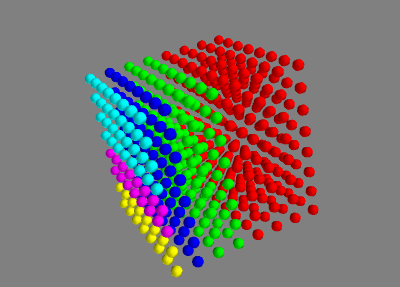
\includegraphics[height=1.2in]{figs/goodallocation}
        \caption{Contiguous}
        \label{fig:overview_sub1}
    \end{subfigure}%
    \hspace{1em}%
    \begin{subfigure}[t]{0.2\textwidth}
        \centering
        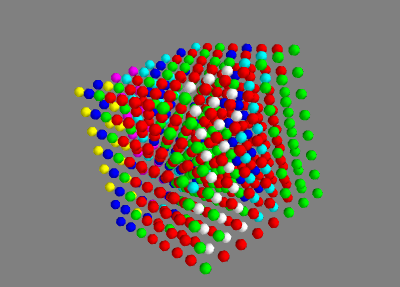
\includegraphics[height=1.2in]{figs/badallocation}
        \caption{Non-contiguous}
        \label{fig:overview_sub2}
    \end{subfigure}%
   \caption{Multiple jobs running concurrently with different allocations. Each job is represented by a specific color. a) shows the effect of contiguous allocation, which reduce the inter-job interference. b) shows non-contiguous allocation, which may introduce both intra and inter-job interferences. }
   \label{fig:overview}
\end{figure}

When submitting jobs to HPC systems, users request resources in terms of node counts and expected runtime. The batch scheduler is then responsible for dispatching the submitted jobs to the system. Typically, multiple jobs run concurrently, resulting in the shared use of resources, particularly network and storage. A prominent problem with this approach is network contention among concurrently running jobs. If the network resources of concurrently running jobs aren't isolated, the resulting sharing can cause communication variability that results in performance degradation for some or all such jobs \cite{abhinav-sc13}. This delay can propagate into the queueing time of the following submitted jobs, thus leading to low system throughput and utilization \cite{jose-ipdps15}. This adverse effect of network sharing can be mitigated by providing jobs with isolated allocations and exclusive network resources.

On the widely used torus-connected HPC systems \cite{bgq,tofu,titan}, two allocation strategies are commonly used. The \emph{contiguous allocation} strategy assigns to each job a compact and contiguous set of computing nodes, as shown in Figure \ref{fig:overview_sub1}. The partition-based allocation approach used in Blue Gene series systems is an example of such a strategy \cite{bgloverview}. The contiguous strategy favors application performance through isolated networking within a partition and the locality that implies. However, this strategy can cause both internal fragmentation (when more nodes are allocated to a job than it requests) and external fragmentation (when sufficient nodes are available for a request, but they can not be allocated contiguously), therefore leading to lower system utilization than is otherwise possible. On the other side of the coin, the \emph{non-contiguous allocation} strategy, used by the Cray XT/XE series \cite{carl-cug}, assigns free nodes to jobs regardless of contiguity, though of course efforts are made to maximize locality. Figure~\ref{fig:overview_sub2} shows an example non-contiguous allocation. While eliminating internal and external fragmentation as seen in contiguous allocation systems, in return non-contiguous allocations introduce contention between jobs due to the interleaving of job nodes. The non-contiguous node allocation can significantly reduce job performance, especially for communication-intensive ones \cite{abhinav-sc13}.

We envision that future HPC schedulers will adopt a flexible job allocation mechanism which combines the best of both contiguous and non-contiguous allocation strategies. Such a flexible mechanism would take shared resource needs of jobs into account when making allocation decisions (e.g., network). With knowledge and analysis of job communication patterns, it can be identified which jobs require network isolation and locality, and to what degree. Then, rather than allocating each job in a ``know-nothing'' manner, one may specialize allocation so that, for example, only the jobs with stringent network needs are given compact, isolated allocations, resulting in maximized utilization and minimized perceivable resource contention effects.

In this work, we focus on an in-depth analysis of intra- and inter-job communication interference with different job allocation strategies on torus-connected HPC systems. Torus-based networks are used on six of the top 10 supercomputers on the June 2015 Top500 lists~\cite{top500}. The current generation of IBM Blue Gene/Q (BG/Q) supercomputers, such as Mira at Argonne Nation Laboratory and Sequoia at Lawrence Livermore National Laboratory, has its nodes connected in a 5D torus network \cite{bgq}. The K computer from Japan uses the ``Tofu'' system, which is a 6D mesh/torus topology \cite{tofu}. Titan, a Cray XK7 supercomputer located at the Oak Ridge Leadership Computing Facility (OLCF), has nodes connected in a 3D torus within the compute partition \cite{titan}. Although our analyses are based on torus networks, the ideas conveyed in this work is applicable to networks with different topologies. 

We selected three signature applications from the DOE Design Forward Project~\cite{designforwardwebpage} as examples to conduct detailed study about their communication patterns. We use a sophisticated simulation toolkit named CODES (standing for Co-Design of Multi-layer Exascale Storage Architectures)~\cite{Jason-2011} as a research vehicle to evaluate the performance of these applications with various allocations in a controlled environment. We then analyze the intra- and inter-job interference by simulating these applications running exclusively and concurrently with different allocations. We believe the insights presented in this work can be very useful for the design of future HPC batch job schedulers and resource managers.


%\NOTE{JJ removed the list of contributions, because they are exactly the same as the preceding paragraph.}
\begin{comment}
The observations of this work are the following:

\begin{itemize}
    \item We study the communication behaviors and identify the communication patterns of three representative HPC applications.
    \item We conduct detailed analysis about the intra- and inter-job interference by running three applications with different allocation strategies. And we find the relation between application's communication pattern and the cause of interference.
    \item We show a novel and flexible way to make allocation with awareness of job's communication pattern, which  is every effective to alleviate the interference between concurrently running jobs. \TODO{do we actually do this, or provide the underpinnings for such a method?}
\end{itemize}

We believe the finds and insights presented in this work would be very useful for the design of future HPC batch job scheduler and resource management module.

\end{comment}

The rest of this paper is organized as follows. Section~\ref{sec:application study} describes the three representative applications from DOE Design Forward Project for our study. Section~\ref{sec:codes} talks about the use of CODES as research vehicle for our work. Section~\ref{sec:config study} shows the performance analysis of three applications on different torus networks. Section~\ref{sec:interference} provides detailed analysis about the intra- and inter-job interference between three applications on torus network with different allocation strategies. Section~\ref{sec:discussion} introduces a path toward communication-pattern aware allocation strategies, given the results of our analysis. Section~\ref{sec:related_work} discusses related work. Finally, the conclusion is presented in Section~\ref{sec:conclusion}.




